\documentclass[10pt, twocolumn]{article}

\usepackage{geometry}
\geometry{left=1.7cm,right=1.7cm, top=1.7cm, bottom=1.7cm}

\setlength{\columnsep}{1cm}

\usepackage{nopageno}


\usepackage{newtxtext}
\usepackage{newtxmath}
\usepackage{courier}

\usepackage{xcolor}

\usepackage[brazil]{babel}

\usepackage{hyperref}
\hypersetup{%
    colorlinks,
    linkcolor={black},
    citecolor={black},
    urlcolor={blue!60!black}
}

\usepackage{booktabs}
\usepackage{adjustbox}

\usepackage[ruled, portuguese, onelanguage]{algorithm2e}
\SetKwBlock{Loop}{loop}{fim}

% ----------------------------
% Updating section headers
\usepackage{titlesec}
% \usepackage{abstract}

\renewcommand{\thesection}{\Roman{section}.}
\titleformat{\section}
{\scshape\centering}{\thesection}{1em}{}

\renewcommand{\thesubsection}{\Alph{subsection}.}
\titleformat{\subsection}
{\itshape}{\thesubsection}{1em}{}

  \renewenvironment{abstract}{%
      \if@twocolumn
        \section*{\abstractname}%
      \else
        \small
        \paragraph{\emph{\abstractname:}}
      \fi}
    %   {\if@twocolumn\else\par\bigskip\fi}


% ----------------------------
% Updating captions
\usepackage{caption}

\captionsetup[table]{labelsep=newline, font={footnotesize, sc}}
\captionsetup[figure]{labelsep=period, font=footnotesize}

% ----------------------------
% Declaring math operations
\usepackage{amsmath}
\DeclareMathOperator*{\argmin}{arg\,min}
\DeclareMathOperator*{\argmax}{arg\,max}

% ----------------------------
% Updating title and authors
\usepackage{titling}
\usepackage{authblk}
\renewcommand\Authand{, }

\pretitle{
    \begin{center}
        \LARGE
}
\posttitle{
    \end{center}
}

\preauthor{
    \fontsize{11}{11}
    \begin{center}
}
\postauthor{
    \par\end{center}
    \vspace{-5em}
    \fontsize{10}{10}
}

\title{Comparação de Algoritmos Heurísticos para o Problema da Coloração de Vértices\vspace{-1ex}}

\author[1]{Lucas Guido}
\author[2]{Caio Stoduto\fontsize{10}{10}\vspace{-1ex}}
\affil[1]{\fontsize{10}{10}CMCC, Universidade Federal do ABC, Santo André -- SP, Brasil  \authorcr
\fontsize{9}{9}\texttt{lucas.guido@aluno.ufabc.edu.br}\fontsize{10}{10}}
\affil[2]{\fontsize{10}{10}CMCC, Universidade Federal do ABC, Santo André -- SP, Brasil \authorcr
\fontsize{9}{9}\texttt{caio.stoduto@aluno.ufabc.edu.br}\fontsize{10}{10}}

\date{}

\begin{document}

\twocolumn[
\maketitle
\begin{@twocolumnfalse}

\noindent
\small
\begin{abstract} 

O Problema da Coloração de Vértices é um problema clássico em grafos.
Ele consiste em colorir o grafo com o menor número possível de cores de modo que
dois vértices adjacentes não compartilhem a mesma cor. Este problema é NP-difícil,
logo, o presente trabalho objetiva estudar a coloração de grafos por meio de heurísticas.
Os algoritmos: \emph{First Fit}, \emph{Welsh Powell}, \emph{Largest Degree Ordering},
\emph{Incidence Degree Ordering}, \emph{Degree of Saturation} e
\emph{Recursive Largest First} foram implementados e suas performances, tanto em
tempo de execução, quanto em qualidade da solução, foram comparadas.

\textit{\textbf{Palavras-Chave:}} Coloração de grafos, Número cromático, Heurísticas, Otimização.
\end{abstract}

\end{@twocolumnfalse}
]

\mdseries
\normalsize
\indent

% \begin{multicols*}{2}
\section{Introdução}

O Problema da Coloração de Vértices, ou \emph{Graph Coloring Problem} (GCP), é
um problema clássico na computação, apesar de postulado muito 
antes do concebimento da ideia de computadores. 
O problema consiste em colorir todos os vértices de um determinado grafo com o 
menor número de cores possível sem que haja nenhum vizinho da mesma cor,
sendo classificado como problema de otimização.
O número mínimo de cores necessárias pra colorir um grafo $G$ é chamado de
número cromático de $G$ e é denotado por $\chi(G)$.

O GCP é um problema NP-difícil~\cite{AsBa18}, de modo que encontrar a solução ótima é uma 
tarefa computacionalmente custosa. 
No entanto, existem algoritmos que tentam abordá-lo de diferentes formas 
para obter um resultado eficiente.
Um exemplo disso são as heurísticas, que se aproveitam das características do 
problema para encontrar soluções boas (e diversas vezes próximas às ótimas)
em um tempo razoável.

O presente artigo aborda o Problema da Coloração de Vértices de grafos utilizando
heurísticas.
Para isso, foram implementados e testados seis algoritmos heurísticos com base no artigo de
Aslan e Baykan~\cite{AsBa18}: \emph{First Fit}~(FF), \emph{Welsh Powell}~(WP),
\emph{Largest Degree Ordering}~(LDO), \emph{Incidence Degree Ordering}~(IDO),
\emph{Degree of Saturation}~(DSATUR) e \emph{Recursive Largest First}~(RLF)~\cite{AsBa18}.

Por fim, os algoritmos são comparados com respeito ao tempo de execução e à
qualidade da solução encontrada.


\section{Algoritmos}

Nesta seção serão apresentados os algoritmos em pseudocódigo.
Todos os seis algoritmos estudados neste artigo são heurísticas determinísticas,
ou seja, não utilizam nenhuma etapa dependente de probabilidade, de modo que
todas as soluções são construídas a partir da estrutura do grafo.

Para os pseudocódigos, são consideradas as seguintes notações:
dado um grafo $G(V,E)$, a cor de um vértice $v \in V$ é denotada por $C(v)$.
Se ainda não foi designada uma cor ao vértice, $C(v) = \textnormal{NULL}$.
Ademais, dado $A \subset V$, $C(A)$ denota o conjunto de cores dos vértices em $A$,
ou seja, $C(A)\nobreak=\nobreak\bigcup_{v \in A} C(v)$. Por fim, o conjunto
$cores = \{c_1, c_2, \dots, c_k\}$ é o conjunto de cores usadas por uma solução,
onde cada $c_i$, para $i = 1, 2, \dots, k$, é uma cor distinta.


% ------------------------------------------
% First Fit Algorithm

\begin{algorithm}
\caption{First Fit (FF)}
\label{alg:ff}

\KwData{Grafo $G(V,E)$}
\KwResult{Coloração de $G$}

\emph{cores} $\gets \emptyset$\;
$n \gets 0$\;
$C(v) \gets$ NULL, $\forall v \in V$\;

\ForEach{$v \in V$} {
    \ForEach{$c \in$ cores} {
        \If{$c \notin C\left(N(v)\right)$} {
            $C(v) \gets c$\;
            break;
        }
    }
    \If{$C(v) = $ \textnormal{NULL}}{
        $n \gets n+1$\;
        \emph{cores} $\gets$ \emph{cores} $\cup \{ c_n \}$\;
        $C(v) \gets c_n$\;
    }
}
\Return{$C$}\;

\end{algorithm}


% ------------------------------------------
% Welsh Powell Algorithm

\begin{algorithm}
\caption{Welsh Powell (WP)}
\label{alg:wp}

\KwData{Grafo $G(V,E)$}
\KwResult{Coloração de $G$}

\emph{cores} $\gets \emptyset$\;
$n \gets 0$\;

$C(v) \gets$ NULL, $\forall v \in V$\;

$U \gets V$\;

\While{$U \neq \emptyset$} {
    $v \gets \argmax_{v \in U} d_G(v)$\;

    $n \gets n + 1$\;
    \emph{cores} $\gets \emph{cores} \cup \{c_n\}$\;

    $C(v) \gets C_n$\;
    $U \gets U \setminus \{v\}$\;

    $V' \gets U \setminus N(v)$\;

    \While{$V' \neq \emptyset$} {
        $v \gets \argmax_{v \in V'} d_G(v)$\;
        
        $C(v) \gets C_n$\;
        $U \gets U \setminus \{v\}$\;

        $V' \gets V' \setminus (\{v\} \cup N(v))$\;
    }
}

\Return{$C$}\;

\end{algorithm}


% ------------------------------------------
% Largest Degree Ordering Algorithm

\begin{algorithm}
\caption{Largest Degree Ordering (LDO)}
\label{alg:ldo}

\KwData{Grafo $G(V,E)$}
\KwResult{Coloração de $G$}

\emph{cores} $\gets \emptyset$\;
$n \gets 0$\;

$C(v) \gets$ NULL, $\forall v \in V$\;
$V' \gets V$\;
Coloque $V'$ em ordem decrescente de graus dos vértices\;

\ForEach{$v \in V'$} {
    \ForEach{$c \in$ cores} {
        \If{$c \notin C(N(v))$}{
            $C(v) \gets c$\;
            break; 
        }
    }
    \If{$C(v) = $ \textnormal{NULL}}{
        $n \gets n+1$\;
        \emph{cores} $\gets$ \emph{cores} $\cup \{ c_n \}$\;
        $C(v) \gets c_n$\;
    }
}
\Return{$C$}\;

\end{algorithm}


% ------------------------------------------
% Incidence Degree Ordering Algorithm

\begin{algorithm}
\caption{Incidence Degree Ordering (IDO)}
\label{alg:ido}

\KwData{Grafo $G(V,E)$}
\KwResult{Coloração de $G$}

\emph{cores} $\gets \emptyset$\;
$n \gets 0$\;
$C(v) \gets$ NULL, $\forall v \in V$\;
$U \gets V$\;

\While{$U \neq \emptyset$}{
    $v \gets \argmax_{v \in U} |N(v) \setminus U|$, em caso de empate, pegue a
    opção de maior grau em $G$.

    \ForEach{$c \in$ cores} {
        \If{$c \notin C(N(v))$}{
            $C(v) \gets c$\;
            break;
        }
    }

    \If{$C(v) = $ \textnormal{NULL}}{
        $n \gets n+1$\;
        \emph{cores} $\gets$ \emph{cores} $\cup \{ c_n \}$\;
        $C(v) \gets c_n$\;
    }

    $U \gets U \setminus \{v\}$\;
}

\Return{$C$}\;

\end{algorithm}


% ------------------------------------------
% Degree of Saturation Algorithm

\begin{algorithm}
\caption{Degree of Saturation (DSATUR)}
\label{alg:dsatur}

\KwData{Grafo $G(V,E)$}
\KwResult{Coloração de $G$}

\emph{cores} $\gets \emptyset$\;
$n \gets 0$\;

$C(v) \gets$ NULL, $\forall v \in V$\;

$U \gets V$\;

\While{$U \neq \emptyset$}{
    $v \gets \argmax_{v \in U} |C(N(v) \setminus U)|$, em caso de empate, pegue a opção de maior grau em $G$.
    
    \ForEach{$c \in$ cores} {
        \If{$c \notin C(N(v))$}{
            $C(v) \gets c$\;
            break;
        }
    }

    \If{$C(v) = $ \textnormal{NULL}}{
        $n \gets n+1$\;
        \emph{cores} $\gets$ \emph{cores} $\cup \{ c_n \}$\;
        $C(v) \gets c_n$\;
    }

    $U \gets U \setminus \{v\}$\;
}
\Return{$C$}\;

\end{algorithm}


% ------------------------------------------
% Recursive Largest First Algorithm

\begin{algorithm}[ht]
\caption{Recursive Largest First (RLF)}
\label{alg:rlf}

\KwData{Grafo $G(V,E)$}
\KwResult{Coloração de $G$}

\emph{cores} $\gets \emptyset$\;
$n \gets 0$\;
$C(v) \gets$ NULL, $\forall v \in V$\;
$V' \gets V$\;
$U \gets \emptyset$\;

\Loop {
    $v \gets \argmax_{v \in V'} |N_{G[V']}(v)|$\;
    $n \gets n + 1$\;
    \emph{cores} $\gets \emph{cores} \cup {c_n}$\;

    \Loop {
        $C(v) \gets C_n$\;
        $V' \gets V' \setminus (\{v\} \cup N(v))$\;
        $U \gets U \cup N(v)$\;

        \If{$V' \neq \emptyset$}{
            $v\nobreak\gets\nobreak \argmax_{v \in V'} |\{(v, k) : k \in \nobreak U \textnormal{ e } (v, k) \in E(G)\}|$\;
            % $v\nobreak\gets\nobreak \argmax_{v \in V'} \left|\{(v, k) \mid k \in U\} \cap E(G)\right|$\;
            continue\;
        }

        \eIf{$\not \exists v \in V \mid C(v) =$ NULL} {
            \Return{$C$}\;
        } {
            $V' \gets U$\;
            $U \gets \emptyset$\;
            break\;
        }
    }
}

\end{algorithm}


\section{Experimentos computacionais}
Nessa seção serão apresentados os resultados obtidos pela implementação.

Os algoritmos foram implementados usando a linguagem C++ e os experimentos foram
rodados em um computador com processador AMD~Ryzen~5~3600XT e com 16 GB de memória,
rodando o sistema operacional Windows~10.
O programa foi compilado usando o GNU GCC.

Para fazer o \emph{benchkmark} dos algoritmos, foram usados grafos da base DIMACS~\cite{dimacs}.
A Tabela~\ref{tab:experiments} apresenta as informações de cada grafo, bem como
os dados da execução de cada algoritmo, identificados pela abreviação do 
algoritmo, que incluem a solução incumbente (K) e o tempo de execução (T), em
milissegundos.
Para obter um tempo de execução consistente, cada algoritmo foi
executado 50 vezes para cada grafo, e foi obtida a média aritmética do tempo
de execução.
Além do mais, a tabela também apresenta a melhor solução conhecida
para cada grafo (Best K). Os valores em negrito indicam que a solução é ótima
(Best K = $\chi(G)$).

\begin{table*}
    \caption{Experimentos computacionais}
    \begin{adjustbox}{width=\textwidth}%
    \small
    \centering
    \begin{minipage}[b]{\textwidth}
        \centering
\begin{tabular}{@{} lrrrrrrrrrrrrrr @{}}
\toprule
& & & \multicolumn{2}{c}{FF} & \multicolumn{2}{c}{WP} & \multicolumn{2}{c}{LDO} & \multicolumn{2}{c}{IDO} & \multicolumn{2}{c}{DSATUR} & \multicolumn{2}{c}{RLF}\\
\cmidrule(lr){4-5}\cmidrule(lr){6-7}\cmidrule(lr){8-9}\cmidrule(lr){10-11}\cmidrule(lr){12-13}\cmidrule(lr){14-15}
Grafo & Vértices & Arestas & K & T (ms) & K & T (ms) & K & T (ms) & K & T (ms) & K & T (ms) & K & T (ms) \\
\midrule
C2000.5 & 2000 & 999836 & 226 & 19.98 & 222 & 7.61 & 222 & 17.55 & 222 & 22.69 & 221 & 20.27 & NaN & NaN \\
C4000.5 & 4000 & 4000268 & 402 & 136.68 & 396 & 28.22 & 396 & 104.60 & 403 & 131.21 & 402 & 119.22 & NaN & NaN \\
dsjc1000.1 & 1000 & 49629 & 31 & 0.24 & 30 & 0.76 & 30 & 0.29 & 30 & 1.29 & 30 & 1.33 & NaN & NaN \\
dsjc1000.5 & 1000 & 249826 & 127 & 3.02 & 124 & 2.00 & 124 & 3.12 & 127 & 4.49 & 127 & 3.85 & NaN & NaN \\
dsjc1000.9 & 1000 & 449449 & 321 & 13.28 & 310 & 3.20 & 310 & 13.72 & 318 & 15.34 & 309 & 14.54 & NaN & NaN \\
dsjc250.5 & 250 & 31336 & 43 & 0.12 & 40 & 0.13 & 40 & 0.12 & 40 & 0.23 & 41 & 0.22 & NaN & NaN \\
dsjc500.1 & 500 & 12458 & 20 & 0.06 & 18 & 0.20 & 18 & 0.07 & 19 & 0.29 & 19 & 0.27 & NaN & NaN \\
dsjc500.5 & 500 & 62624 & 72 & 0.48 & 69 & 0.48 & 69 & 0.55 & 70 & 0.76 & 71 & 0.75 & NaN & NaN \\
dsjc500.9 & 500 & 224874 & 175 & 1.94 & 168 & 0.83 & 168 & 2.10 & 174 & 2.85 & 176 & 2.91 & NaN & NaN \\
dsjr500.1c & 500 & 121275 & 109 & 0.58 & 99 & 0.51 & 99 & 1.13 & 101 & 1.46 & 97 & 1.45 & NaN & NaN \\
dsjr500.5 & 500 & 58862 & 143 & 0.99 & 133 & 0.72 & 133 & 1.33 & 129 & 1.53 & 133 & 1.64 & NaN & NaN \\
flat1000-50-0 & 1000 & 245000 & 126 & 2.85 & 121 & 2.05 & 121 & 2.85 & 122 & 3.97 & 122 & 3.83 & NaN & NaN \\
flat1000-60-0 & 1000 & 245830 & 125 & 2.99 & 124 & 2.01 & 124 & 2.99 & 123 & 4.03 & 124 & 3.90 & NaN & NaN \\
flat1000-76-0 & 1000 & 246708 & 122 & 2.80 & 123 & 1.99 & 123 & 2.87 & 125 & 4.31 & 123 & 3.72 & NaN & NaN \\
flat300-28-0 & 300 & 21695 & 46 & 0.18 & 46 & 0.19 & 46 & 0.17 & 49 & 0.26 & 46 & 0.24 & NaN & NaN \\
latin-square & 900 & 307350 & 213 & 3.44 & 155 & 1.46 & 155 & 5.02 & 147 & 6.21 & 158 & 5.68 & NaN & NaN \\
le450-25c & 450 & 17343 & 37 & 0.11 & 31 & 0.24 & 31 & 0.15 & 30 & 0.32 & 32 & 0.31 & NaN & NaN \\
le450-25d & 450 & 17425 & 35 & 0.11 & 30 & 0.26 & 30 & 0.14 & 31 & 0.32 & 33 & 0.33 & NaN & NaN \\
r1000.1c & 1000 & 485090 & 138 & 2.14 & 117 & 1.31 & 117 & 3.70 & 124 & 5.25 & 116 & 4.64 & NaN & NaN \\
r1000.5 & 1000 & 238267 & 275 & 6.80 & 259 & 3.04 & 259 & 9.68 & 250 & 10.03 & 253 & 10.03 & NaN & NaN \\
r250.5 & 250 & 14849 & 79 & 0.20 & 71 & 0.17 & 71 & 0.25 & 69 & 0.28 & 71 & 0.28 & NaN & NaN \\
\bottomrule
\end{tabular}
\end{minipage}
\end{adjustbox}
\end{table*}

O gráfico da Fig.~\ref{fig:boxplot} apresenta a acurácia de cada algoritmo com
relação à melhor solução conhecida.
Para calcular a acurácia de cada algoritmo para cada grafo, foi usada a fórmula
$A=K_{B}/K_A$, onde $K_{B}$ é a melhor solução conhecida para o grafo e
$K_A$ é a solução incumbente de cada algoritmo.



A partir do gráfico da Fig.~\ref{fig:boxplot}, é possível observar que o algoritmo
\emph{First Fit} resultou nas piores soluções, enquanto o \emph{Recursive Largest First}
foi o melhor, com uma média de 80\% do \emph{Best K} e chegando a uma acurácia de 93\%.
Os outros algoritmos tiveram todos soluções de qualidade parecida, entre FF e RLF
e com acurácia média por volta de 70\%.

Apesar de diversos algoritmos possuírem soluções de alta acurácia (acima de 90\%),
é importante notar que nenhum atingiu o \emph{Best K}, indicando que existem
alternativas melhores.

\begin{figure}[ht]
  \centering
  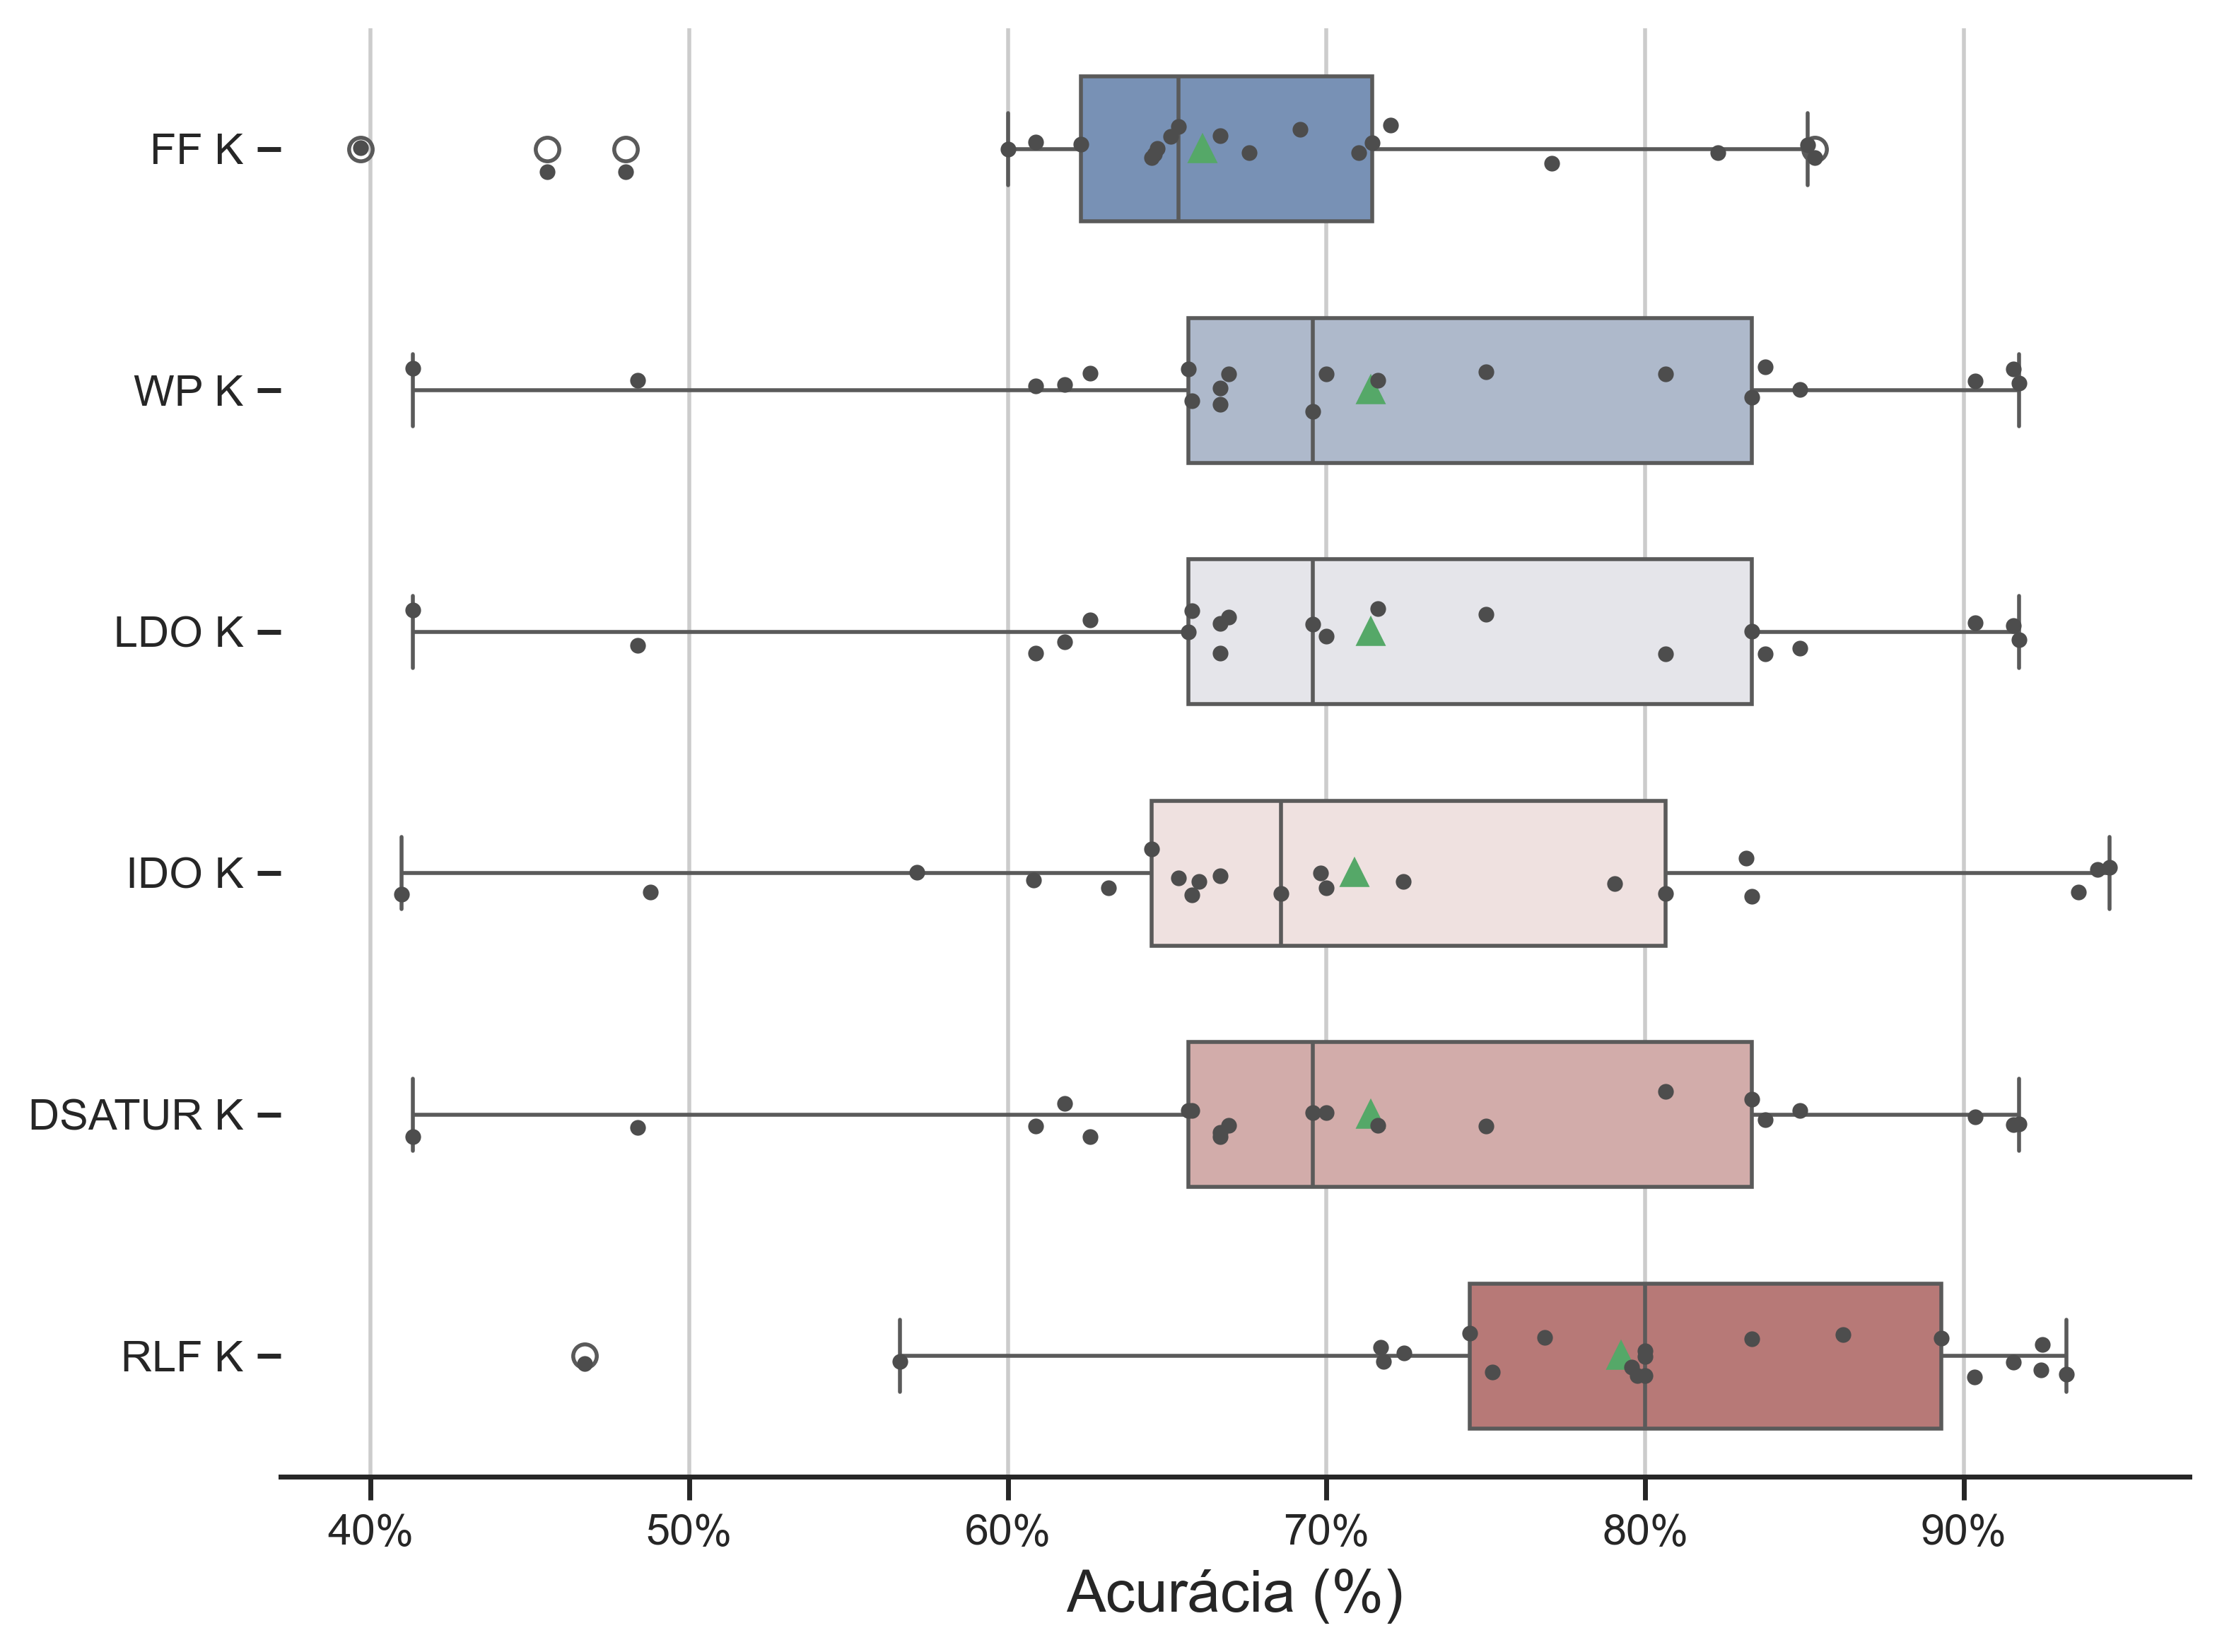
\includegraphics[scale=0.42]{img/boxplot.png}
  % \caption{Gráfico da porcentagem de instâncias de acordo com a distância mínima para b(G)}
  \caption{Boxplot indicando a acurácia das soluções incumbentes encontradas por
  cada algoritmo em relação ao melhor valor conhecido.
  O eixo $x$ indica a acurácia, enquanto que o eixo $y$ indica os algoritmos.
  O triângulo verde indica a média da acurácia do modelo.
  }
  \label{fig:boxplot}
\end{figure}

Em quesito de tempo, o RLF foi consistentemente o mais lento, o que pode ser
justificado pela qualidade superior das soluções.
O DSATUR também apresentou execução mais lenta comparado aos outros, indicando
que este algoritmo não é uma boa escolha para os grafos usados no \emph{benchmark},
pois produziu soluções de qualidade similar a outros com tempo de execução muito menor.



\section{Conclusão}
Observando a performance dos algoritmos para o problema de GCP, é possível concluir
que o algoritmo RLF obtém a média com maior acurácia, chegando até a $93.23\%$ nos
grafos de \emph{benchmark}. Contudo, levando em consideração o tempo de execução
de cada algoritmo, a longa duração de execução do RLF deve ser levada em consideração,
já que é discrepantemente mais lento que os outros algoritmos.

\bibliographystyle{amsplain}
\bibliography{bibliography.bib}

% \end{multicols*}

\end{document}